%\documentclass[journal,10pt]{article}
\documentclass[journal,10pt]{IEEEtran}
\usepackage{hyperref}
\usepackage{todonotes}
\usepackage{amssymb}
\usepackage{amsmath}
\usepackage{mathtools}
\usepackage{graphicx}

\newcommand{\subtask}[1]{\begin{quote}\textbf{#1}\end{quote}}
\newcommand{\hod}{h}
\newcommand{\moh}{m}
\newcommand{\dow}{d}
\newcommand{\dom}{d_m}
\newcommand{\wom}{w_m}
\newcommand{\woy}{w_y}
\newcommand{\yyy}{a}

\newcommand{\IN}{\mathbb{N}}
\newcommand{\defeq}{\coloneqq}

\author{Jan Lippert \(<\)\href{mailt:ljan@mail.upb.de}{ljan@mail.upb.de}\(>\)}
\date{\today}

\begin{document}

\title{Predicting Parking Space Availability in Paderborn}
\maketitle

\begin{abstract}
The Parking Prediction system Paderborn is available at \url{http://pppb.herokuapp.com/}. It was written in Play! Scala and uses the \href{smile}{haifengl.github.io/smile/} library. It was planned to predict the number of available parking spaces for the ``Libori-Galerie'' 15 minutes in advance, e.g. loading the web page in the browser will show the prediction. Currently, this functionality was not implemented yet as the quality of predictions is insufficient. Alternative models need to be investigated and implemented for the final system. 
\end{abstract}

\section{Topic introduction}

\subsection{Previous Intro 1}

In urban areas, space and as such parking space is limited. Car owners often have to drive around to available parking spots. This leads to an unnecessary waste of time and additional air pollution. 

According to multiple studies, the availability of parking data reduces the search time for a parking spot \cite{Asakura1994}\cite{Caicedo2010228}. However, most systems only provide the current number free parking spots. In rush hours, this information can quickly get outdated and lead to driving around to find available parking spaces.

%\cite{parkendd} is a similar project which shows the current free parking spots in different cities. This information is collected from different websites. In addition, \cite{parkendd} collected data over the course of a year and used machine learning to predict the usage of the covered car park ``Centrum Galerie''\footnote{\url{http://mechlab-engineering.de/2015/03/vorhersage-der-parkhausbelegung-mit-offenen-daten/}}. 
%\cite{Rajabioun2013} and \cite{Zheng2015} propose similar systems to predict the availability of parking space to help car owners find a parking spot in advance. 

In Paderborn the situation is similar: live-data is available but no prediction. The proposed project will collect parking data from Paderborn and use machine learning to predict the number of free parking spots.

\subsection{Previous Intro 2}
In urban areas, space and as such parking space is limited. Car owners often have to drive around to available parking spots. This leads to an unnecessary waste of time and additional air pollution. 

According to multiple studies, the availability of parking data reduces the search time for a parking spot \cite{Asakura1994}\cite{Caicedo2010228}. However, most systems only provide the current number free parking spots. In rush hours, this information can quickly get outdated and lead to driving around to find available parking spaces.

The goal of this project is to predict the available parking space in advance. Because of the limitation outlined in \ref{sec:challenged}, we will focus on the covered car park ``Libori-Galerie''. This car park is also the most interesting as it is directly connected to a local shopping center. It is opened from 06:00 am to 02:00 am.

\subsection{Previous Intro 3}
In urban areas, space and as such parking space is limited. Car owners often have to drive around to available parking spots. This leads to an unnecessary waste of time and additional air pollution. 

According to multiple studies, the availability of parking data reduces the search time for a parking spot \cite{Asakura1994}\cite{Caicedo2010228}. However, most systems only provide the current number free parking spots. In rush hours, this information can quickly get outdated and lead to driving around to find available parking spaces.

This report will describe how such a system could be implemented. Section \ref{sec:architecture} will show how the overall architecture of the system will look like. Section \ref{sec:frameworks} will compare the different frameworks that were considered for the implementation. 


\subsection{What question does your work answer}

\subsection{What related work does exist}

\subsection{Why did you choose your topic}



\subsection{Related Work}
\cite{parkendd} is a similar project which used the collected data to predict parking space availability. This project focussed on the car park ``Centrum Galerie''. \cite{parkendd} used the following features: week of year, day of week, time of day, sunday openings and the number of workdays until the next public holiday. Sunday openings are used as in Germany, shops are normally closed on Sundays. Sunday openings therefore influence how many people go to the shopping center and therefore the availability of parking space. In \cite{parkendd}, different algorithms are compared and the predictions are evaluated.

\cite{Rajabioun2013} propose parking guiding and
information system which also includes the prediction of available parking space. The proposed algorithm uses a probabilistic model based on historical data. Among others, the used features also include time of day and day of week. At last, \cite{Rajabioun2013} estimates the mean-error on predictions. They mention that predictions for 10 minutes in the future lead to a 1.2\% error on average while predictions for 40 minutes in the future lead to a 2.8\% error on average.

\cite{Zheng2015} compared three different feature sets and three different machine learning algortihms -- regression tree, neural network, and support vector regression -- with respect to their performance. Based on data from the cities of Melbourne and San Francisco they conclude that the regression tree provides the best predictions when used with a feature set containing day of week and time of day.  



\subsection{Data Sources}\label{data sources}
The main data source is the actual parking data which is available online. In addition there are other possible features that influence parking space availability. Since taking all features into account is not possible, this project will focus on the parking data and optionally extend the model with basic event data.

\paragraph{Parking Usage Live Data}
The homepage of the ASP Paderborn\footnote{City-Managed service for waste management, city cleaning, and parking.} lists the city managed parking areas and the number of currently free parking spots. 
The data is available on \url{https://www.paderborn.de/microsite/asp/parken_in_der_city/freie_Parkplaetze_neu.php}. A more minimal website is available at \url{https://www4.paderborn.de/ParkInfoASP/default.aspx}. 

Since there is no API known, the parking data needs to be scraped from the website.  
\paragraph{Event Data (Optional)}
A second data source could be public holidays and local events. In some cases, these events influence the number of free parking spots directly: the Libori fair is located on the parking area ``Le Mans Wall'' and the ``Lunapark'' is located on ``Maspernplatz''. 

Other events may also cause more people to go to the city center and therefore to more parking space usage. One example includes Sunday openings. In Germany, shops are normally closed on Sunday. Howevery, cities may choose to allow shopping on a few Sundays a year. 

This data is considered optional as the big events do not happen while the course ``Practical Project in Machine Learning'' takes place. A list of these events can be found on the homepage of the carneval club\footnote{\url{http://www.kirmes-paderborn.de/termine.htm}}. The city's homepage also lists some events\footnote{\url{https://www.paderborn.de/tourismus-kultur/veranstaltungen/veranstaltungshighlights.php}}. Both of these sources would have to be parsed manually.



\section{Feasibility}

To keep the scope of this project small, multiple data sources will be ignored. For this project, it is assumed that the number of available parking spots solely depends on time. As described in \ref{data sources}, this obviously is a very simplified model. However, as shown by \cite{parkendd}, such a simple model may be enough. 

The greatest challenge in this project is to collect enough training data to make meaningful predictions. All data needs to be extracted from APS's website. Changes to the website and non-availability of the service may prove problematic. In the beginning of February, the ASP parking guiding system was dysfunctional and did not show useful data online. 

The next limit is the usage of heroku's free plan. This plan limits the used database to 10000 rows. When crawling every 15 minutes, this limits the amount of available training data to roughly one week; the amount can be increased, since the 10000 row limit can be exceeded for 7 days before new inserts into the database are disabled.


\section{Model}
\subtask{Describe your selected model training method and discuss the reasoning behind your selection.}
\subsection{Training Methods} 

\section{Verification}
\subtask{Describe and discuss your ``objective method'', ie. the method by which you will measure the success of your predictor.}
To verify the trained model and the accuracy of its predictions, the predictions will be queried in regular intervals and compared to the actual available parking space at that time. 

\section{Methodology choice}

\subsection{Introduction of chosen methodology}

\subsection{Motivation behind choice}

\subsection{Discussion of possible problems with data or methodology}
\paragraph{Initial results}
\paragraph{Investigation of alternative methologies}

\subsection{Comparison between methodologies, if applicable}
\paragraph{Comparison of results}

\subsection{Final choice of methodology}

\section{Previous report}


%%%%%%%%%%
%
% Methdology Start
%
%%%%%%%%%%

\section{Data Sources}\label{data sources}
The main data source is the actual parking data which is available online. In addition there are other possible features that may influence parking space availability. Since taking all features into account is not possible, this project will solely focus on the parking data in relation to time. 

\paragraph{Parking Usage Live Data}
The homepage of the ASP Paderborn\footnote{City-Managed service for waste management, city cleaning, and parking.} lists the city managed parking areas and the number of currently free parking spots. 
The data is available on \url{https://www.paderborn.de/microsite/asp/parken_in_der_city/freie_Parkplaetze_neu.php}. A more minimal website is available at \url{https://www4.paderborn.de/ParkInfoASP/default.aspx}. 

The website displays 4 attributes: name, type, capacity, and available spots\footnote{respectively: Parkstätte, --, Anzahl, Frei}. After crawling, the parking information will be annotated with the crawling time. The latter will be split into multiple attributes which will be used in the prediction: hour of day \(\hod\), minute of hour \(\moh\), day of week \(\dow\), day of month \(\dom\), week of month \(\wom\), week of year \(\woy\), and \(\yyy\)\footnote{the year is included as a way to keep samples unique in case the project runs more than 1 year.}.

The number of available parking spaces is be called \(y\). With the features defined before, the training data will be a set of tuples of the form  
\[
(\hod, \moh, \dow, \dom, \wom, \woy, \yyy, y)\text{.}
\]

\paragraph{Event Data (Optional)}
As mentioned in the first report, public holidays and local events could influence the parking situation near the city center. In some cases, these events take place \textit{on} one of the parking areas. However, as most of the big events do not happen while the course ``Practical Project in Machine Learning'' takes place, we will not consider them further.

\begin{figure}
  \centering
  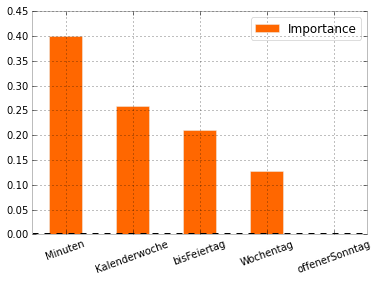
\includegraphics[scale=0.5]{parkendd-Feature-Importance.png}
  \caption{Importance of Features (ParkenDD)}
  \label{fig:parkendd_features}
\end{figure}

Public holidays like Christmas and Easter may also influence the availability of parking space. \cite[parkendd] modelled this in the feature ``bisFeiertag'', i.e. working days until public holiday. In figure \ref{fig:parkendd_features}, the relevance of the different features used by \cite{parkendd} is displayed\footnote{respectively: minutes, week of year, working days until public holiday, day of week, Sunday openings}. 

The feature was relatively important in the evaluation done by \cite{parkendd}. Nonetheless, it will not be included as the next public holiday is Christi Himmelfahrt on 25th May 2017. Therefore there would be no possibility of verifying the importance of this feature in time.

\paragraph{Weather Data (Optional)}

Weather data may also prove to be useful for prediction as, e.g., more people may decide to take the car when it's raining. Weather data is available online, e.g. at \url{https://openweathermap.org/api}. Weather data will not be considered in the prediction to keep the model simpler.


\section{Hypothesis}

It is assumed, that the available parking space is dependent on time, i.e. there exists a function \(f\) such that 
\[
f(\hod, \moh, \dow, \dom, \wom, \woy, \yyy) = y\text{.}
\]



\section{Feasibility}

To keep the scope of this project small, multiple data sources will be ignored. For this project, it is assumed that the number of available parking spots solely depends on time. As described in \ref{data sources}, this obviously is a very simplified model. However, as shown by \cite{parkendd}, such a simple model may be enough. 

The greatest challenge in this project is to collect enough training data to make meaningful predictions. All data needs to be extracted from APS's website. Changes to the website and non-availability of the service may prove problematic. In the beginning of February, the ASP parking guiding system was dysfunctional and did not show useful data online. 

The next limit is the usage of heroku's free plan. This plan limits the used database to 10000 rows. When crawling every 15 minutes, this limits the amount of available training data to roughly one week; the amount can be increased, since the 10000 row limit can be exceeded for 7 days before new inserts into the database are disabled.


\section{Model}
\subtask{Describe your selected model training method and discuss the reasoning behind your selection.}
\subsection{Training Methods} 

\section{Verification}
\subtask{Describe and discuss your ``objective method'', ie. the method by which you will measure the success of your predictor.}
To verify the trained model and the accuracy of its predictions, the predictions will be queried in regular intervals and compared to the actual available parking space at that time. 

%%%%%%%%%%
%
% Methdology End
%
%%%%%%%%%%


\section{Run-time technology}

\subsection{Introduction of run-time system}

\subsection{Technology choices and motivation}

\subsection{Discussion of possible problems with setting up run-time system}

\subsection{Previous report}

%%%%%%%%%%%
%
% Technology Start
%
%%%%%%%%%%%

\subsection{Architecture}\label{sec:architecture}
One important part in the choice of technology was the separation of the different concerns in the applications. There are multiple parts that play together: crawling, preprocessing, training, prediction, and finally evaluation. 

Crawling has to be done on a regular basis. Therefore the chosen framework needs to support regular execution of jobs. When new entries are crawled, they are cleaned via the preprocessing module and inserted in the database. Since it may be necessary to update the model over time, the preprocessing module will also have a regular job that cleans existing entries by updating them to the most recent model.



\subsection{Frameworks}\label{sec:frameworks}
To implement this project, Ruby on Rails, Python and Scala were considered. I used Ruby on Rails in previous projects and development is quite fast with this framework. However, I could only find a few libraries that deal with machine learning \cite{bigml} \cite{leanpanda}. 
Another choice of language was python. Python has quite a lot pf machine learning libraries and is also used in academics. However, I do not have much previous experience with python.

My final choice was the \href{Play! framework}{https://playframework.com} with Scala. I did use this framework in previous projects and therefore was familiar with setting up background jobs and how to enable web access. Heroku also supports easy deployment for Play! applications\todo{insert links in final report}. One important factor of this choice was the type-safety of the Scala language and it's usage in machine learning and big data\todo{insert link in final report}. While the problem at hand is certainly not big data, the multitude of existing libraries helped a lot to get started\todo{add links to the libraries in final report}.

I chose to use \href{Smile}{http://haifengl.github.io/smile/index.html}, the ``Statistical Machine Intelligence and Learning Engine''. It was easy to use and documentation is quite extensive. In some cases, the API documentation even references the scientific papers the learning algorithm is based on. 


\section{Encountered Problems}
\subsection{Malfunction of the Parking Guidance System}
One week after the first prototype of the crawler was online, \url{https://www.paderborn.de/microsite/asp/parken_in_der_city/freie_Parkplaetze_neu.php} was non-functional. The number of available parking spaces for the ``Liborie-Galerie'' was always set to \(0\).

At the same time, many of the other parking areas were switched to ``Nicht im Parkleitsystem'' (not part of the parking guidance system). Both of these issues were caused by a malfunction of the parking guidance system. Crawling was resumed normally after the parking guidance system was fixed by the provider.

On another note, string values were not expected for the Liborie-Galerie. This caused the crawler to crash on every crawl; the crawler was then adapted to be ore resilient to unexpected values: all non-integer values for free spaces will directly be dropped.

\subsection{Heroku Free Dyno Limitations}

After collecting data for some time, I did some correlation analysis on the data. I noticed that all entries had ``\(\wom = 1\)'' despite the app being online for more than a week. Further investigation showed that the data was only available for 3 different days. 

The reason for this failure was the uninformed use of the Heroku Free package. Free dynos will sleep after 30 minutes minutes of inactivity. After this was noticed, multiple services and workarounds were investigated.

However, most of the workarounds were from before 2015. In 2015, Heroku added the requirement that free dynos need to sleep 6 hours a day. Unfortunately the most promising service -- \url{http://kaffeine.herokuapp.com/} -- is not functional anymore.

To keep the system running, a bash script was created which keeps the dyno awake by sending regular HEAD requests. Since the dyno is still required to sleep 6 hours a day, a sleeping time had be chosen. Luckily, the ``Libori-Galerie'' is closed from 2am to 8am and the dyno will rest in this period. 

\subsection{Free Database Limitations}
At first, there were multiple problems in accessing the database The free tier only allows 20 concurrent connections to the Postgresql database. These connections were exhausted 5 minutes after the start of the application. This could be solved by configuring the application to restricting the number of database connections to 10 -- when the application was configured to use 20 connections, problems persisted.

The next limit is in the size of the database. The free tier only allows \(10000\) rows. Insert actions will be disabled after the database has had more than \(10000\) for 7 days. This challenge will be circumvented by removing old data in regular intervals.



\section{Performance}
As initially expected, the prediction accuracy is quite low. The regression tree has a mean absolute error of \(106.09\) when using \(754\) training examples and \(83\) test examples. The currently best result was achieved by using a Random Forest Classificator; using the same examples as before, the RFC had a mean absolute error of \(64.36\). This clearly shows that model and training method have to improved by a great deal before actually becoming useful. 

To do so, the next part of the project will consist of trying out different models and experimenting with other features. Live predictions will be added soon with the warning that they are experimental and probably not usable yet.



%%%%%%%%%%%
%
% Technology End
%
%%%%%%%%%%%

\section{Results}

\subsection{Result of your work (hypothesis statement)}

\subsection{Discussion of possible future work}

\subsection{Reflection against existing literature}



\section{Reflection}

\subsection{What did you learn}


\bibliographystyle{ieeetr}  
\bibliography{report_lippert}

\end{document}
